\documentclass[11pt]{article}

\usepackage[margin=1in]{geometry}
\usepackage{hyperref}
\usepackage{tikz}
\usepackage{booktabs}
\usepackage{enumitem}
\usepackage{xcolor}
\usepackage{listings}
\usepackage{parskip}
\usepackage{pdflscape}
\usetikzlibrary{positioning, arrows.meta, shapes.geometric, fit, backgrounds}

\hypersetup{
  colorlinks=true,
  linkcolor=black,
  urlcolor=blue!60!black,
  citecolor=black
}

\lstset{
  basicstyle=\ttfamily\footnotesize,
  frame=single,
  framesep=4pt,
  breaklines=true,
  columns=fullflexible,
  keepspaces=true,
  showstringspaces=false
}

\title{\textbf{Polaris Orders}\\\large Schema, Domain, and First Vertical Slice}
\author{Ahmed Khan}
\date{\today}

\begin{document}
\maketitle

\begin{abstract}
\noindent This document describes the concrete design of the order subsystem: how the \texttt{orders} table is shaped, how the \texttt{Order} domain type is derived from it, how the identifier scheme splits internal UUIDs from customer-facing order numbers, and what exists in code today versus what is planned.

General architectural principles behind these choices --- the rationale for layered design, why Domain and Persistence are peers rather than a stack, the event-log pattern, and related references --- live in \texttt{docs/architecture.md}. Contributor-facing code conventions live in \texttt{docs/contributing.md}. Order-number design details live in \texttt{docs/order-numbers.md}.
\end{abstract}

\section{Architecture of the Order Slice}

The order code is split across four layers, with the Service composing Domain and Persistence from above. The Domain is a leaf: nothing depends downstream of it.

\begin{center}
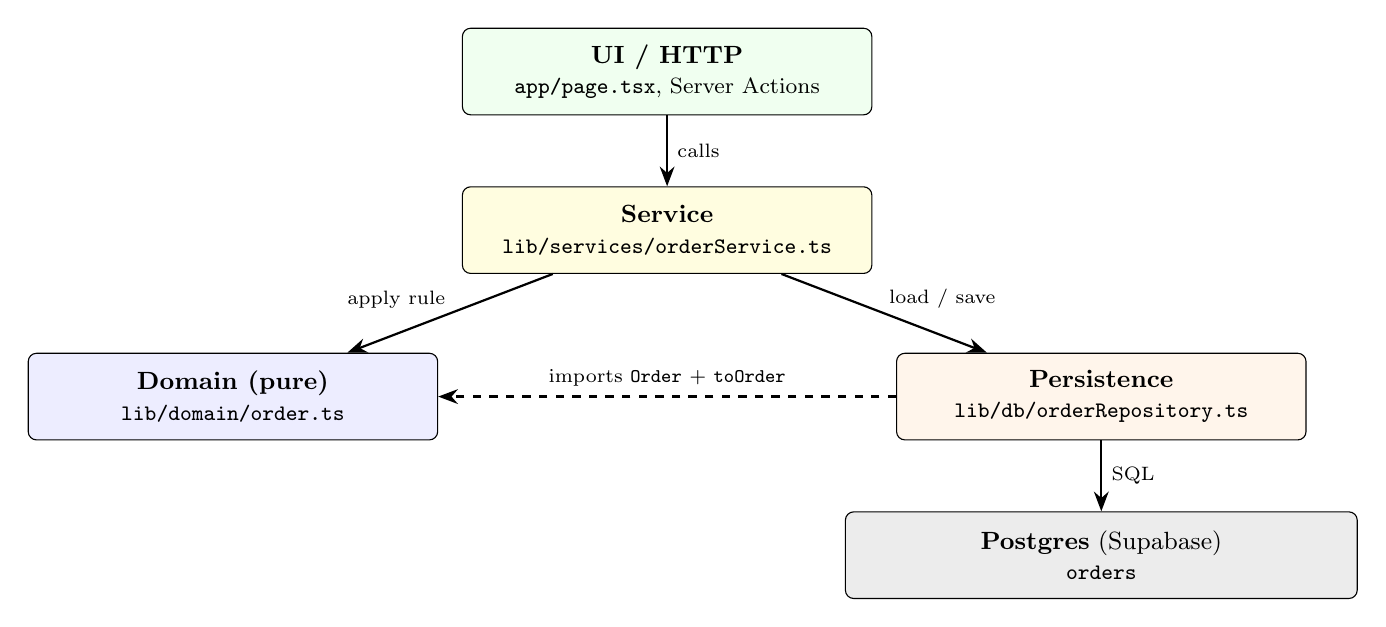
\begin{tikzpicture}[
  node distance=0.9cm and 1.2cm,
  box/.style={draw, rounded corners=3pt, minimum width=5.2cm, minimum height=1.1cm, align=center, font=\small},
  ui/.style={box, fill=green!6},
  service/.style={box, fill=yellow!12},
  pure/.style={box, fill=blue!7},
  impure/.style={box, fill=orange!8},
  db/.style={box, fill=gray!15, minimum width=6.5cm},
  arrow/.style={-{Stealth[length=2.5mm]}, thick}
]

\node[ui] (ui) {\textbf{UI / HTTP}\\\footnotesize\texttt{app/page.tsx}, Server Actions};
\node[service, below=of ui] (service) {\textbf{Service}\\\footnotesize\texttt{lib/services/orderService.ts}};
\node[pure, below left=1.0cm and 0.3cm of service] (domain) {\textbf{Domain (pure)}\\\footnotesize\texttt{lib/domain/order.ts}};
\node[impure, below right=1.0cm and 0.3cm of service] (persist) {\textbf{Persistence}\\\footnotesize\texttt{lib/db/orderRepository.ts}};
\node[db, below=of persist] (db) {\textbf{Postgres} (Supabase)\\\footnotesize\texttt{orders}};

\draw[arrow] (ui) -- (service) node[midway, right, font=\scriptsize] {calls};
\draw[arrow] (service) -- (domain) node[midway, above left=-0.1cm, font=\scriptsize] {apply rule};
\draw[arrow] (service) -- (persist) node[midway, above right=-0.1cm, font=\scriptsize] {load / save};
\draw[arrow] (persist) -- (db) node[midway, right, font=\scriptsize] {SQL};
\draw[arrow, dashed] (persist) -- (domain) node[midway, above, font=\scriptsize] {imports \texttt{Order} + \texttt{toOrder}};

\end{tikzpicture}
\end{center}

\noindent\textbf{Dependency rule.} UI depends on Service; Service depends on Domain and Persistence; Persistence depends on Drizzle, the database, and --- narrowly --- the Domain (dashed arrow) for the \texttt{Order} type and \texttt{toOrder} mapper. The Domain depends on nothing. Every arrow points \emph{toward} the Domain. The rationale for this shape and the alternatives considered are in \texttt{docs/architecture.md}.

\begin{landscape}
\section{Layer Responsibilities in the Order Slice}

Each layer has a contract: what code is allowed to live in it, what is forbidden, and which other layers it may call. Crossings of this contract are review-time red flags.

\begin{center}
\begin{tabular}{@{}p{2.4cm}p{3.6cm}p{3.6cm}p{3.6cm}p{3.6cm}p{3.6cm}@{}}
\toprule
 & \textbf{UI} & \textbf{Service} & \textbf{Domain} & \textbf{Persistence} & \textbf{Database} \\
\midrule
\textbf{Lives here} & rendering, actions & orchestration, transactions & types, pure functions & queries, mapping & tables, constraints, sequences \\[6pt]
\textbf{Forbidden} & rules, SQL & SQL & I/O, randomness & rules & --- \\[6pt]
\textbf{May call} & Service, Persistence & Domain, Persistence & --- & Drizzle, Domain & --- \\
\bottomrule
\end{tabular}
\end{center}

\noindent Two subtleties worth naming. First, \textbf{Persistence depends on Domain}: the repository imports both the \texttt{Order} type (as a contract for what it must return) and the \texttt{toOrder} mapper (its projection function). Both are pure and depend on nothing below, so the import is narrow and inward-pointing --- it does not compromise Domain's status as a leaf. Second, \textbf{reads may skip the Service}: a Server Component rendering a list may call the repository directly, because there is no domain rule to apply and the repository already returns domain-shaped objects. Mutations always go through the Service so any future rule has a natural hook to land in.
\end{landscape}

\begin{landscape}
\section{Mutation Flow for Future Order Operations}

Three-beat rhythm: \textbf{load} $\to$ \textbf{apply} $\to$ \textbf{save}. Rules live in Domain, I/O in Persistence, sequencing in Service.

\medskip
\noindent\emph{Status today.} The flow below is the pattern order mutations will grow into. The only mutation currently wired (\texttt{createOrder}) bypasses load/apply because creation has no precondition to enforce --- a UUID is generated and the row is inserted. The load $\to$ apply $\to$ save shape becomes necessary once status transitions arrive (see \texttt{docs/roadmap.md}).

\begin{center}
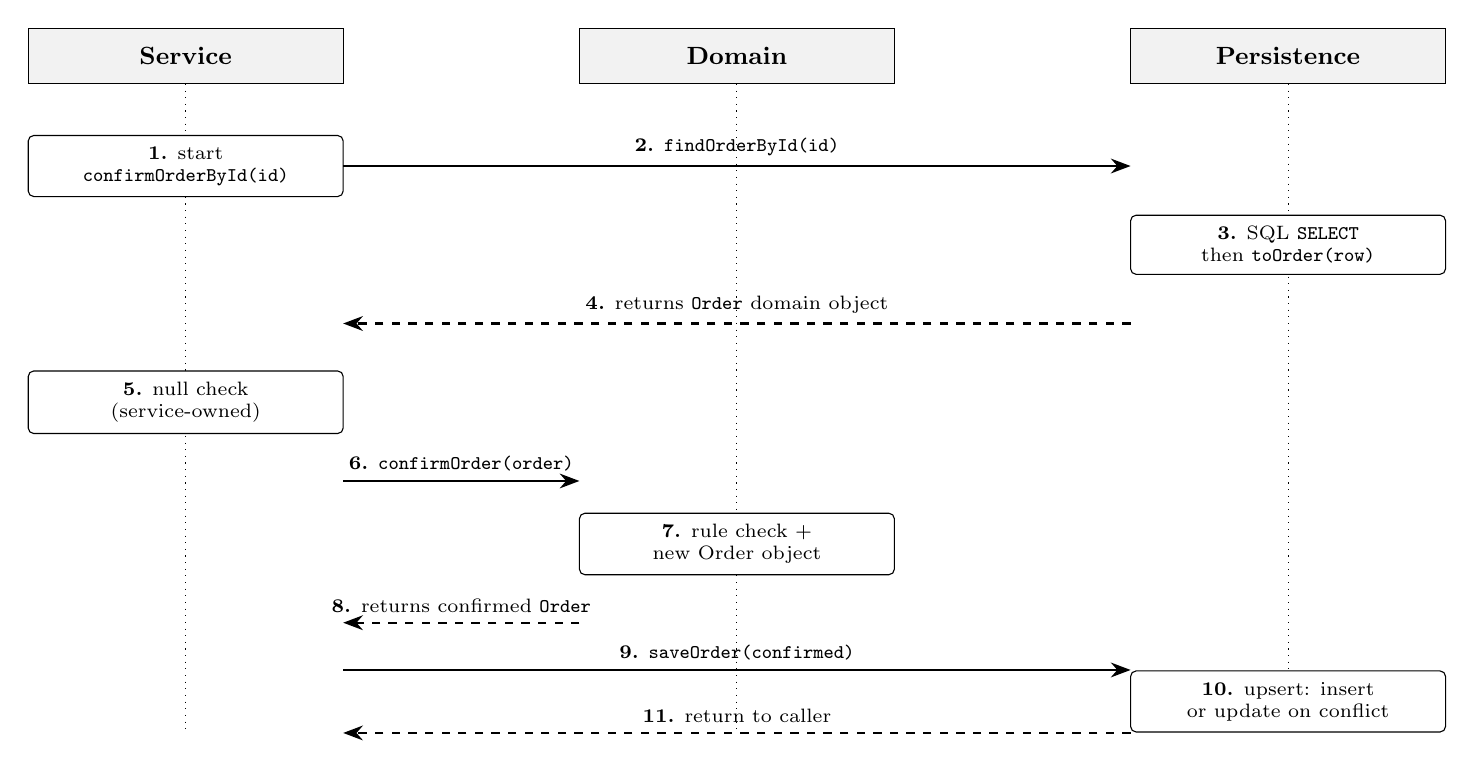
\begin{tikzpicture}[
  node distance=2.4cm,
  lane/.style={draw, minimum width=4cm, minimum height=0.7cm, font=\small\bfseries, fill=gray!10},
  stepbox/.style={draw, rounded corners=2pt, font=\scriptsize, align=center, inner sep=4pt, fill=white, minimum width=4cm},
  arrow/.style={-{Stealth[length=2.5mm]}, thick},
  ret/.style={-{Stealth[length=2.5mm]}, thick, dashed}
]

\node[lane] (svcH) at (0,0) {Service};
\node[lane] (domH) at (7,0) {Domain};
\node[lane] (perH) at (14,0) {Persistence};

\draw[dotted] (svcH) -- ++(0,-8.6);
\draw[dotted] (domH) -- ++(0,-8.6);
\draw[dotted] (perH) -- ++(0,-8.6);

\node[stepbox] (s1) at (0,-1.4) {\textbf{1.} start\\\texttt{confirmOrderById(id)}};
\draw[arrow] (2,-1.4) -- (12,-1.4) node[midway, above, font=\scriptsize] {\textbf{2.} \texttt{findOrderById(id)}};

\node[stepbox] (s3) at (14,-2.4) {\textbf{3.} SQL \texttt{SELECT}\\then \texttt{toOrder(row)}};
\draw[ret] (12,-3.4) -- (2,-3.4) node[midway, above, font=\scriptsize] {\textbf{4.} returns \texttt{Order} domain object};

\node[stepbox] (s5) at (0,-4.4) {\textbf{5.} null check\\(service-owned)};

\draw[arrow] (2,-5.4) -- (5,-5.4) node[midway, above, font=\scriptsize] {\textbf{6.} \texttt{confirmOrder(order)}};
\node[stepbox] (s7) at (7,-6.2) {\textbf{7.} rule check +\\new Order object};
\draw[ret] (5,-7.2) -- (2,-7.2) node[midway, above, font=\scriptsize] {\textbf{8.} returns confirmed \texttt{Order}};

\draw[arrow] (2,-7.8) -- (12,-7.8) node[midway, above, font=\scriptsize] {\textbf{9.} \texttt{saveOrder(confirmed)}};
\node[stepbox] (s10) at (14,-8.2) {\textbf{10.} upsert: insert\\or update on conflict};
\draw[ret] (12,-8.6) -- (2,-8.6) node[midway, above, font=\scriptsize] {\textbf{11.} return to caller};

\end{tikzpicture}
\end{center}

\noindent Solid arrows are calls; dashed are returns. Steps 3 and 10 touch SQL; steps 6--7 are the only pure-logic beats.
\end{landscape}

\section{First Vertical Slice}

\subsection{Current State}

The Order domain is deliberately minimal --- just enough to prove the architecture and exercise the order-number generation scheme. One mutation (\texttt{createOrder}), one query (\texttt{findAllOrders}), a single pure function (\texttt{toOrder} mapping DB rows to the domain shape), and a read-only Server Component rendering a four-column Kanban over seeded orders. Status, transitions, customers, and line items are deferred; see \texttt{docs/roadmap.md}.

\begin{lstlisting}[language={}]
type Order = {
  id: string          // UUID, internal primary key, never rendered to users
  orderNumber: number // bigint, customer-facing, from Postgres sequence
  createdAt: Date     // server-set via DEFAULT now()
}
\end{lstlisting}

\subsection{Identifier Scheme}

Every order carries two identifiers with different jobs. \texttt{id} is a UUID --- a good database key: unguessable, generatable without a round-trip, unaffected by ordering. \texttt{orderNumber} is a \texttt{bigint} sourced from a Postgres sequence \texttt{order\_number\_seq} starting at \texttt{1\_000\_000} --- a good human identifier: short, pronounceable, barcode-friendly, the thing dispatchers read over a radio. Neither compromises for the other's role. The application never generates an order number; the database does, via \texttt{DEFAULT nextval('order\_number\_seq')}. Full rationale and constraints live in \texttt{docs/order-numbers.md}.

\subsection{File Map}

\begin{center}
\begin{tabular}{@{}p{6cm}p{8cm}@{}}
\toprule
\textbf{File} & \textbf{Role} \\
\midrule
\texttt{lib/domain/order.ts} & \texttt{Order} type + \texttt{toOrder} mapper (pure) \\
\texttt{lib/db/orderRepository.ts} & Drizzle queries; imports \texttt{toOrder} \\
\texttt{lib/services/orderService.ts} & \texttt{createOrder} (insert only, no domain rule yet) \\
\texttt{lib/schema.ts} & Drizzle schema: \texttt{orders} + \texttt{order\_number\_seq} \\
\texttt{lib/db.ts} & Drizzle client setup \\
\texttt{lib/seed.ts} & Development seed data \\
\texttt{app/page.tsx} & Server Component rendering the Kanban \\
\texttt{app/actions.ts} & \texttt{createOrderAction} Server Action + \texttt{revalidatePath} \\
\texttt{drizzle/0001..0003\_*.sql} & Incremental migrations (posts$\to$orders; trim columns; add uuid + sequence) \\
\texttt{tests/migrations.test.ts} & Testcontainers-backed migration smoke test \\
\texttt{tests/orderMapper.test.ts} & Unit tests for \texttt{toOrder} (incl.\ leak guard) \\
\bottomrule
\end{tabular}
\end{center}

\end{document}
